\documentclass{presentation}

\title{The Role of Electronics Shops}
\subtitle{In a Research Environment}
\author{Blaise Thompson}

\institute{University of Wisconsin--Madison}
\date{2024-04-10}

\begin{document}
\maketitle

\section{Research Shops}

\begin{frame}\frametitle{UW-Madison Department of Chemistry}
  Current shop.
\end{frame}

\begin{frame}\frametitle{UW-Madison Department of Chemistry}
  Historical context.
\end{frame}

\begin{frame}\frametitle{Electronics Shops}
  At other institutions... purdue.. u wash
\end{frame}

\section{Custom Research Electronics}

\begin{frame}\frametitle{Projects}
  Some of our projects
\end{frame}

\section{Electrical Safety}

\begin{frame}\frametitle{Humility}
  Shop staff are not safety experts.
  \vfill
  Thank YOU ALL.
\end{frame}

\section{Thank You}

\begin{frame}\frametitle{Thank You}
  \begin{columns}
    \begin{column}{0.33\textwidth}
      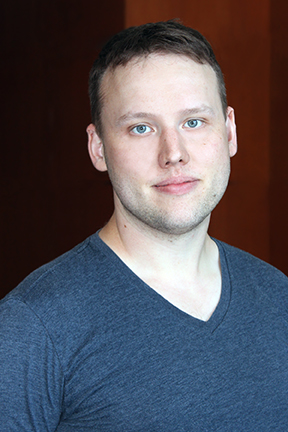
\includegraphics[width=\textwidth]{"./Thompson_Blaise_LowRes.jpg"}
    \end{column}
    \begin{column}{0.67\textwidth}
      Blaise Thompson \\
      Chemistry Electronics Shop \\
      blaise.thompson@wisc.edu
      \vskip 3 em
      We are here to help you use electrical equipment in your research.
      Please reach out!
      \vskip 3 em
      \hl{Questions?}
    \end{column}
  \end{columns}
\end{frame}

\end{document}
